\documentclass[11pt,notes=hide,aspectratio=169,mathserif]{beamer}

% PACKAGES
\usepackage{graphics}
\usepackage{graphicx}  % \resizebox
\usepackage{url}
%\usepackage{natbib}
\usepackage{bibentry}
\usepackage{verbatim}
\usepackage{booktabs}
\usepackage{etoolbox}
\usepackage{datetime}
\usepackage{bm}
\usepackage{subcaption}
\usepackage{amsfonts}
\usepackage{amsmath}
\usepackage{amsthm}

% CUSTOM DEFINITIONS
\def\newblock{} % Get beamer to cooperate with BibTeX
\linespread{1.2}

% IDENTIFYING INFORMATION
\title[class]{ECON 340: Economics of the Family \\ TA Session 1}
\author[vaidehi's class ]{Vaidehi Parameswaran (Northwestern Economics)}
\date{\monthname[\the\month] \the\year}

% THEME OPTIONS
\usetheme{metropolis}
\definecolor{mycolor}{RGB}{48,7,144}
\setbeamercolor{frametitle}{bg=mycolor, fg=white}
\setbeamercolor{title separator}{fg=mycolor}
\setbeamercolor{progress bar}{fg=mycolor}
\beamertemplatenavigationsymbolsempty
\setbeamertemplate{footline}[frame number]{}
\setbeamertemplate{itemize item}{\small\raisebox{1pt}{\textcolor{mycolor}{$\blacktriangleright$}}}
\setbeamertemplate{itemize subitem}{\footnotesize\raisebox{1pt}{\textcolor{mycolor}{$\triangleright$}}}
\setbeamertemplate{itemize subsubitem}{\tiny\raisebox{1pt}{\textcolor{mycolor}{$\triangleright$}}}

% Clickable links
\usepackage{hyperref}
\hypersetup{
  colorlinks=true,
  linkcolor=mycolor,
  urlcolor=mycolor,
  citecolor=mycolor
}

% BACKUP SLIDE NUMBERING
\usepackage{appendixnumberbeamer}

% Show a bulleted mini-contents slide at each section
% Bulleted ToC using your triangle icons + color
\setbeamertemplate{section in toc}{%
  \leavevmode\llap{\textcolor{mycolor}{$\blacktriangleright$}\hspace{0.6ex}}%
  \inserttocsection\par}
\setbeamertemplate{subsection in toc}{%
  \leavevmode\llap{\textcolor{mycolor}{$\triangleright$}\hspace{1.1ex}}%
  \inserttocsubsection\par}

\AtBeginSection[]{
  \begin{frame}{Today}
    \tableofcontents[currentsection]
  \end{frame}
}

\begin{document}

%---------------------------------------------------------------------
\begin{frame}[plain]
\titlepage
\end{frame}
%---------------------------------------------------------------------

\section{Introductions}
%---------------------------------------------------------------------
\begin{frame}{Introductions}
\begin{itemize}
  \item Me: a third-year grad student in the econ department
  \begin{itemize}
    \item Interested in labour, gender, development
    \item Email: \textcolor{blue}{vaidehiparameswaran2029@u.northwestern.edu}
    \item Office hours: Tuesday 11--12pm, Friday 12--1pm in KGH 3411
  \end{itemize}
\end{itemize}
\end{frame}
%---------------------------------------------------------------------

%---------------------------------------------------------------------
\begin{frame}{Why Family?}
\begin{itemize}
  \item The roles of family and culture have been historically ignored in mainstream economics
  \item But family is central to economic questions. Why?
  \pause \item Family decisions affect labour supply, savings, and investment in children
  \pause \item Families are the main channel for transmission of culture and values, which affect economic behaviour
\end{itemize}
\end{frame}
%---------------------------------------------------------------------

\begin{frame}{Four Themes}
\begin{itemize}
  \item Family institutions vary across space and time — the nuclear family is not the only way to organise family life.
  \item Intergenerational transmission of ideas and beliefs
  \item Social beliefs that govern family practices —such as marital payments, inheritance, and co-residence upon marriage— are key determinants of economic decision-making in both high- and low-income countries.
  \item Culture is not immutable; it evolves with technological, economic, and policy changes.
\end{itemize}
\end{frame}
%---------------------------------------------------------------------

\begin{frame}{Definitions}
\begin{itemize}
  \item \textbf{Family}: “A family can be defined as the smallest group of individuals who see themselves as connected to one another... Families tend to reside together and share economic opportunities and other rights and responsibilities.”
  \item \textbf{Culture}: “The customary beliefs, social forms, and material traits of a racial, religious, or social group.”
\end{itemize}
\end{frame}
%---------------------------------------------------------------------

\section{Family Institutions}
%---------------------------------------------------------------------
\begin{frame}{Large variation even in traditional cultural traits}
\begin{itemize}
  \item Patrilocality
  \begin{figure}
    \centering
    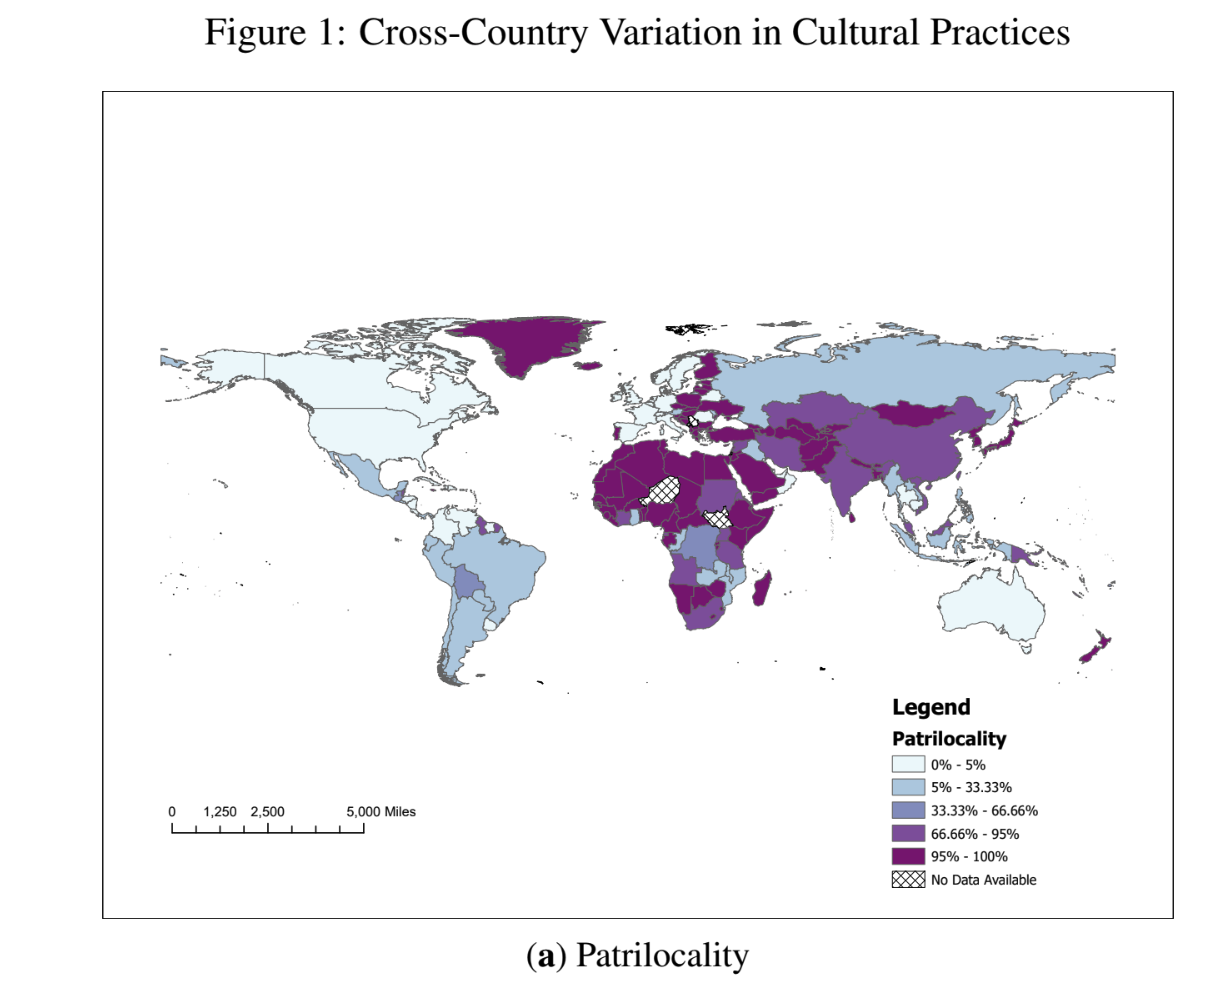
\includegraphics[width=0.6\textwidth]{patri.png}
  \end{figure}
\end{itemize}
\end{frame}
%---------------------------------------------------------------------

\begin{frame}{Large variation even in traditional cultural traits}
\begin{itemize}
  \item Bride price
  \begin{figure}
    \centering
    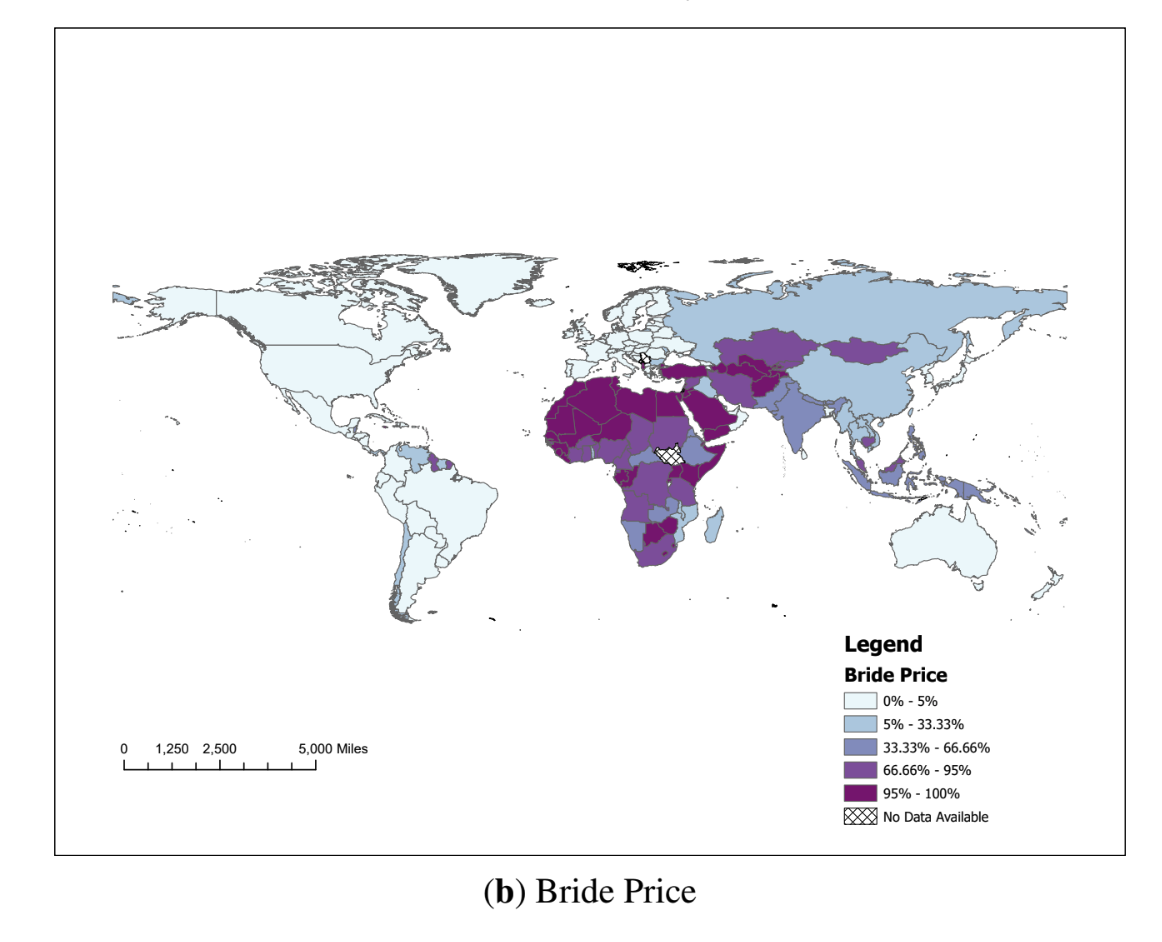
\includegraphics[width=0.6\textwidth]{brideprice.png}
  \end{figure}
\end{itemize}
\end{frame}
%---------------------------------------------------------------------

\begin{frame}{Large variation even in traditional cultural traits}
\begin{itemize}
  \item Polygyny
  \begin{figure}
    \centering
    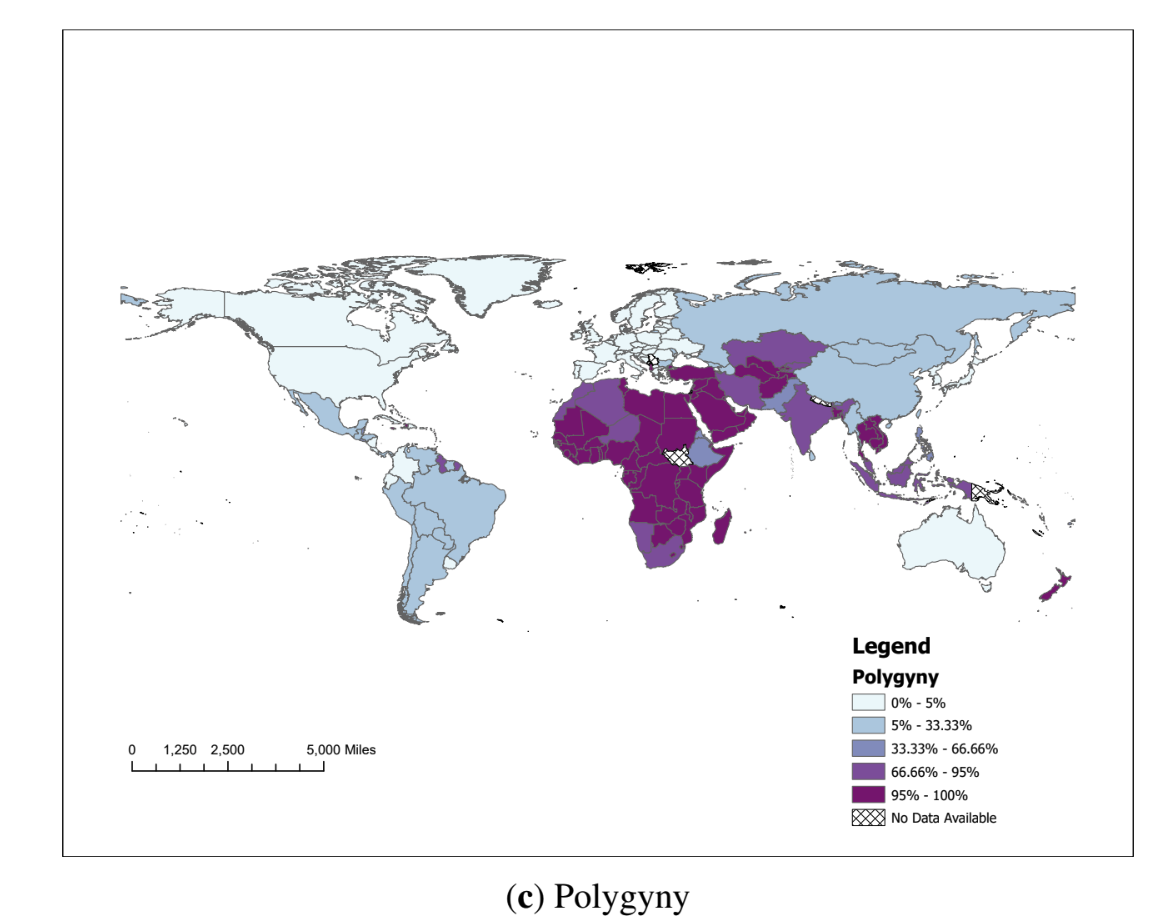
\includegraphics[width=0.6\textwidth]{polygyny.png}
  \end{figure}
\end{itemize}
\end{frame}
%---------------------------------------------------------------------

\begin{frame}{Large variation even in traditional cultural traits}
\begin{itemize}
  \item Nuclear family
  \begin{figure}
    \centering
    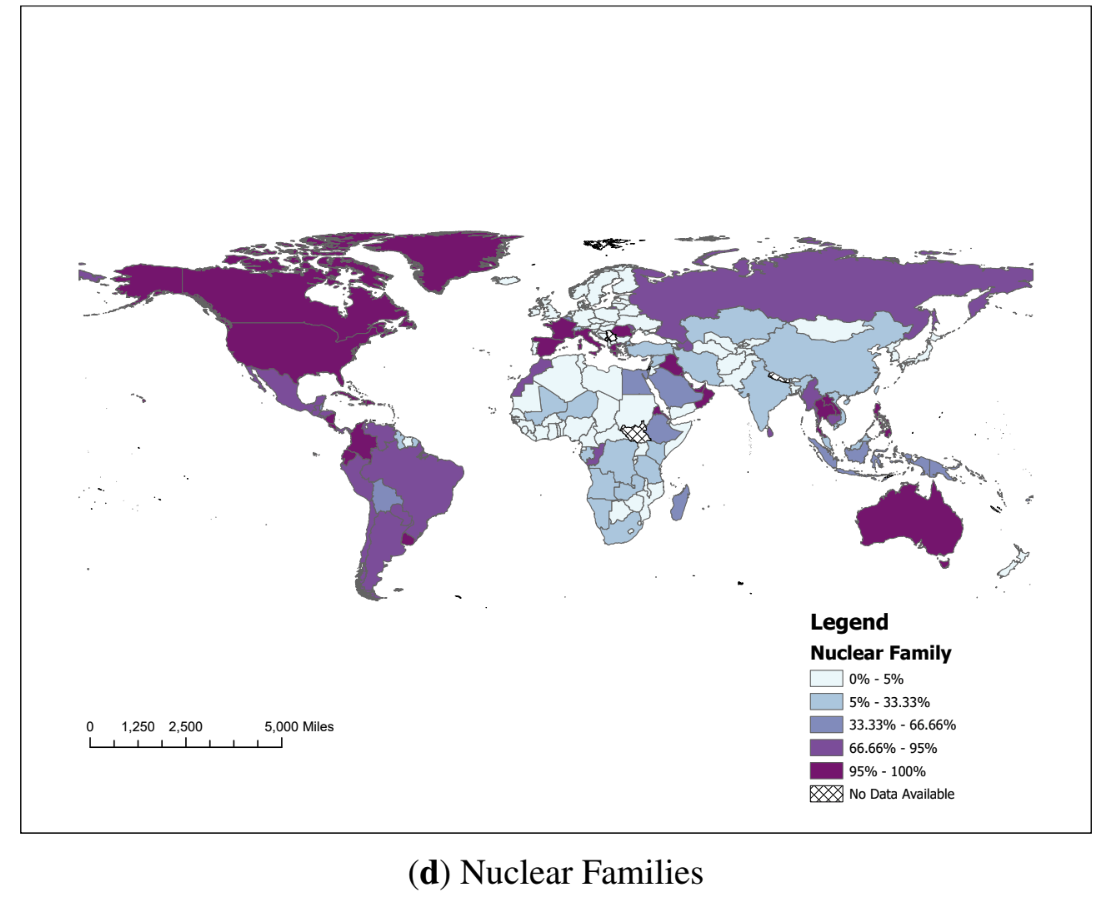
\includegraphics[width=0.6\textwidth]{nuclear.png}
  \end{figure}
\end{itemize}
\end{frame}
%---------------------------------------------------------------------

\begin{frame}{Why do traditional family institutions vary?}
\begin{itemize}
  \item Largely an open question in economics
  \item Cultural institutions can:
  \begin{itemize}
    \item Act as decision-making heuristics.
    \item Shape beliefs and attitudes.
    \item Set the “rules of the game”.
    \item Act as equilibrium selection mechanisms.
  \end{itemize}
  \item They can also be evolutionary responses to environment—agro-climatic conditions and technologies
\end{itemize}
\end{frame}
%---------------------------------------------------------------------

%---------------------------------------------------------------------
\begin{frame}{Evidence}
\begin{itemize}
  \item Becker (2021): historical pastoralism leads to more restrictions on women's sexuality.
  \item Alesina et al. (2013): strength-based pre-industrial agricultural technology contributed to male dominance and a strong division of gender responsibilities.
  \item Boserup (2007): societies relying on labour-intensive, small-tool agriculture show greater prevalence of polygyny and bride price.
\end{itemize}
\end{frame}
%---------------------------------------------------------------------

\begin{frame}{Modern changes}
\begin{itemize}
  \item The second demographic transition: \pause decline in fertility, later marriage, marital instability, cohabitation.
  \item Why? 
  \pause \item Self-actualisation (Lesthaeghe (2010)).
  \item Mismatch between gender attitudes at home and the labour market (Goldscheider et al. (2015) and Esping-Andersen and Billari (2015)).
  \item Natural instability that should fade with the second half of the gender revolution—men involved in home production—already observed in Sweden.
\end{itemize}
\end{frame}
%--------------------------------------------------------------------

%---------------------------------------------------------------------
\begin{frame}{Evolution of Total Fertility Rates}
\begin{figure}
  \centering
  \begin{subfigure}{0.48\textwidth}
    \centering
    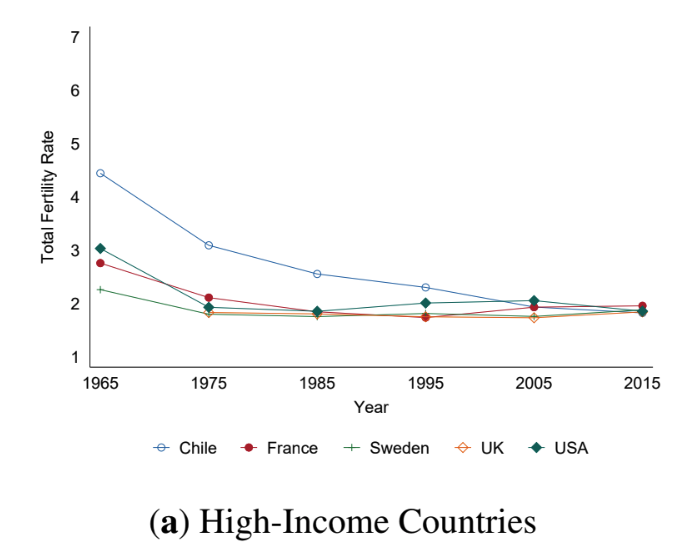
\includegraphics[width=\linewidth]{hic.png}
  \end{subfigure}\hfill
  \begin{subfigure}{0.48\textwidth}
    \centering
    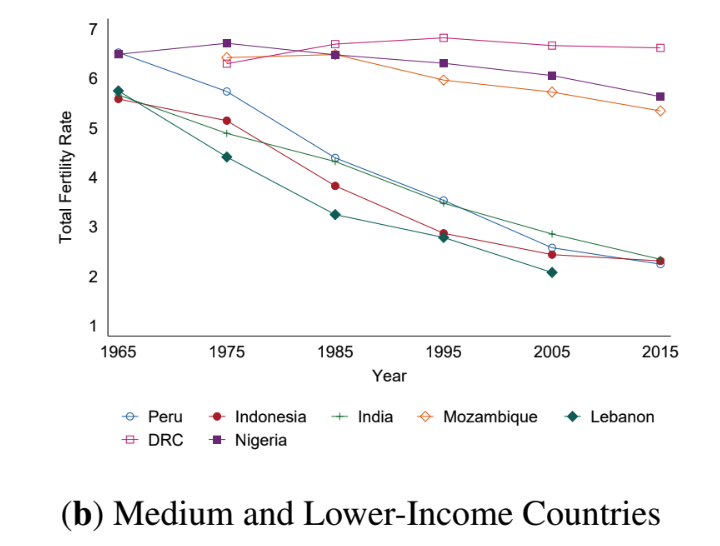
\includegraphics[width=\linewidth]{mlic.png}
  \end{subfigure}
\end{figure}
\end{frame}
%---------------------------------------------------------------------

%---------------------------------------------------------------------
\begin{frame}{Evolution of Divorce Rates}
  \begin{figure}
    \centering
    \begin{subfigure}{0.48\textwidth}
      \centering
      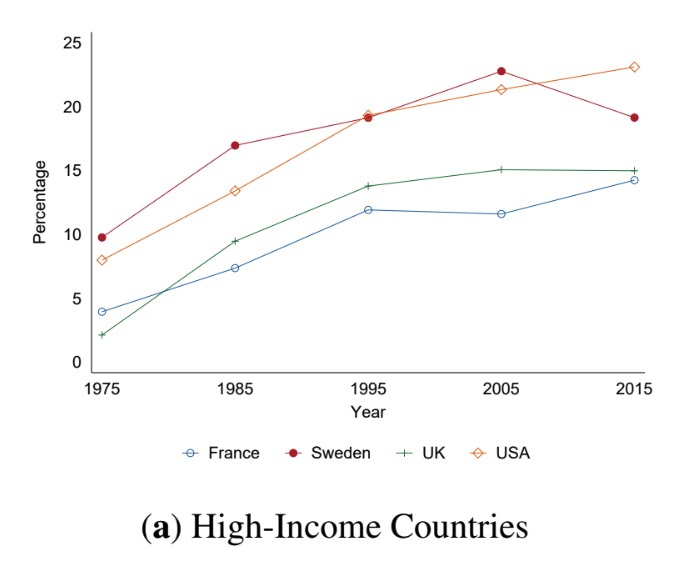
\includegraphics[width=\linewidth]{hic_divorce.png}
    \end{subfigure}\hfill
    \begin{subfigure}{0.48\textwidth}
      \centering
      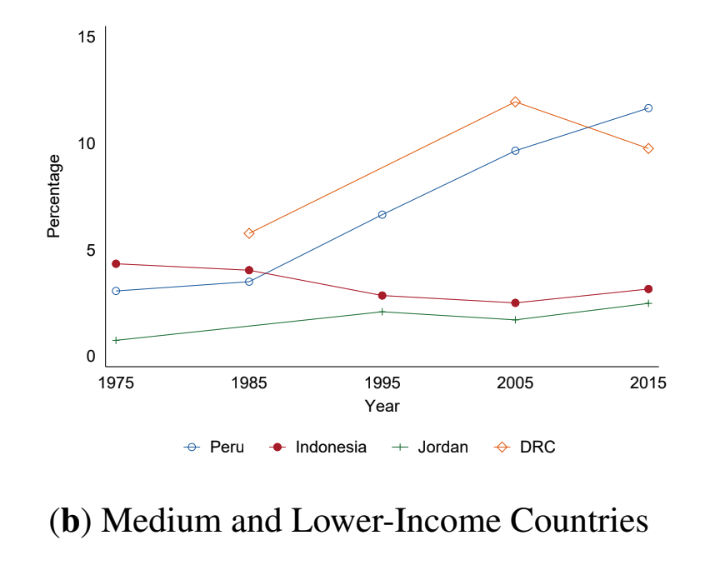
\includegraphics[width=\linewidth]{mlic_divorce.png}
    \end{subfigure}
  \end{figure}
  \end{frame}
  %---------------------------------------------------------------------
  

%---------------------------------------------------------------------
\begin{frame}{Other changes}
\begin{itemize}
  \item Cohabitation has increased—for social and economic reasons.
  \item Open questions—stability of cohabitation vs marriage; who is choosing to cohabit vs marry; intergenerational consequences.
  \item The rise of same-sex couples
  \begin{figure}
    \centering
    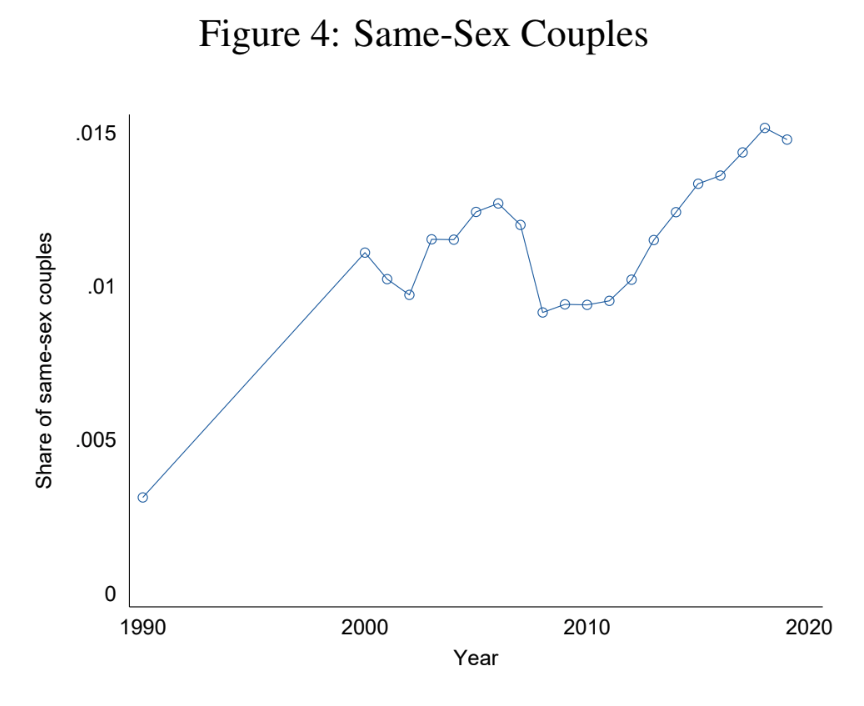
\includegraphics[width=0.5\textwidth]{same_sex.png}
  \end{figure}
\end{itemize}
\end{frame}
%---------------------------------------------------------------------

\section{The Family \& the Transmission of Culture}
%---------------------------------------------------------------------
\begin{frame}{Female LFP and Fertility — Fernandez and Fogli (2009)}
\begin{itemize}
  \item Research question: How does culture affect women's labour force participation and fertility behaviour?
  \item Use the 1970 US Census to create a sample of second-generation married American women aged 30--40.
  \item Census question: “In what country were your parents born?”
  \item Use 1950 TFR and FLFP as proxies for culture.
  \item Controls: MSA of residence, education, household income, parental education, human capital in ethnic group.
  \item Main result: ancestral FLFP predicts women’s work hours and ancestral TFR predicts number of children.
\end{itemize}
\end{frame}
%---------------------------------------------------------------------

\begin{frame}{Historical Family Arrangements}
\begin{itemize}
  \item Todd (1983): four types of family:
  \begin{itemize}
    \item absolute nuclear family: no strict inheritance rules, independent living
    \item egalitarian nuclear family: egalitarian inheritance, independent living
    \item stem family: cohabitation, non-egalitarian inheritance
    \item communitarian family: cohabitation, collective ownership
  \end{itemize}
  \item Galasso and Profeta (2018): these family types predict pension systems that countries adopt.
  \item Egalitarian societies have shared responsibility for supporting parents, so they also support more generous pension systems.
\end{itemize}
\end{frame}
%---------------------------------------------------------------------

\section{How Does Culture Affect Family Decision-Making?}
%---------------------------------------------------------------------
\begin{frame}{Marriage Payments}
\begin{itemize}
  \item \textbf{Dowries}: payments from the bride's family to the groom's family, practised in South Asia and India.
  \item \textbf{Bride prices}: payments from the groom's family to the bride's family, practised in regions of Africa.
  \item Economists' take: “market-clearing transfers”.
\end{itemize}
\end{frame}
%---------------------------------------------------------------------

\begin{frame}{Literature on Marriage Payments}
\begin{itemize}
  \item Ashraf et al. (2020):
  \begin{itemize}
    \item Study the effect of bride price on parents' human capital investments in daughters.
    \item Show that higher bride price payments are associated with greater female education.
    \item Ethnic groups that practised bride price had daughters more likely to be enrolled in school, relative to groups that did not.
    \item Use exogenous school construction programmes in Indonesia and Zambia as sources of variation.
  \end{itemize}
  \item Bhalotra et al. (2020):
\end{itemize}
\end{frame}
%---------------------------------------------------------------------

\begin{frame}{Literature on Marriage Payments}
\begin{itemize}
  \item Ashraf et al. (2020):
  \item Bhalotra et al. (2020):
  \begin{itemize}
    \item Exploit the fact that dowry is paid in gold.
    \item Thus, fluctuations in gold prices affect dowry payments; they hypothesise that increases in gold prices lead to stronger son preference.
    \item They find that prior to 1985, positive gold price shocks increased neonatal mortality of girls but not boys.
    \pause \item After 1985, increases in gold price led to more male-skewed sex ratios.
    \pause \item Why 1985? Sex-selective abortion technologies became widely available.
  \end{itemize}
\end{itemize}
\end{frame}
%---------------------------------------------------------------------

%---------------------------------------------------------------------
\begin{frame}{Son Preference}
\begin{itemize}
  \item Male-biased behaviour: patrilocality, patrilineality, female “purity” norms, cultural rites performed by men.
  \item In extreme forms: female infanticide, sex-selective abortion, abandonment, lower investments.
  \item Technologies can amplify son preference—ultrasound, IVF—see Chen et al. (2013).
\end{itemize}
\end{frame}
%---------------------------------------------------------------------

\begin{frame}{Literature on Son Preference}
\begin{itemize}
  \item Effects on investments:
  \begin{itemize}
    \item Jayachandran and Pande (2017): use son preference to explain stunting differences between India and regions of Africa.
    \item At a given level of income, Indians are much shorter, yet outperform on other health and development indicators.
    \item Prenatal investments are higher for second-born female children with no older brother before gender is observed, but postnatal investments after gender is observed are lower.
  \end{itemize}
  \item Drivers of son preference: inheritance laws.
  \begin{itemize}
    \item Bhalotra et al. (2019): effects of a land reform in West Bengal that increased productivity and strengthened property rights; the reform increased male child survival rates in families without a firstborn son.
  \end{itemize}
\end{itemize}
\end{frame}
%---------------------------------------------------------------------

\begin{frame}{Intimate Partner Violence (IPV)}
\begin{itemize}
  \item In developed countries such as the US, surveys show that 37\% of women report experiencing IPV over their lifetimes.
  \item Beyond immediate negative consequences, women affected by IPV are more likely to develop mental health problems, alcohol and substance abuse, unintended pregnancies, and employment difficulties.
  \item IPV is also associated with negative outcomes for children—lower birth weights and negative externalities on their peers.
\end{itemize}
\end{frame}
%---------------------------------------------------------------------

\begin{frame}{Cash Transfers and IPV — Baranov et al. (2021)}
\begin{itemize}
  \item A household bargaining model.
  \item Violence affects: man's utility, relative status, bargaining power, woman's productivity in the home and in the market.
  \item Cash transfer to a woman: $\uparrow$ her bargaining power, $\downarrow$ his status—ambiguous effects.
  \item Violence may decrease if the transfer relaxes the budget constraint and increases her outside option.
  \item But it may increase to restore his status or to extract resources.
  \item Meta-analyses generally find reductions in IPV.
\end{itemize}
\end{frame}
%---------------------------------------------------------------------

\section{Conclusion}
%---------------------------------------------------------------------
\begin{frame}{Conclusion and Open Questions}
\begin{itemize}
  \item Effects of policies and shocks depend critically on culture, family institutions, and beliefs.
  \item Family institutions are diverse and still changing.
  \begin{itemize}
    \item Why do different institutions arise and change?
    \item How do/did societies establish who has the authority to decide whom a child marries or with which parent children should reside in the case of separation/divorce?
    \item How should we understand the role of the state in shaping family institutions?
  \end{itemize}
  \item Technological change, policy and institutional changes, learning, and exogenous shocks:
  \begin{itemize}
    \item How does the introduction of incentives for taking parental leave (e.g., Sweden and Norway) change the division of work in the household, child-rearing responsibilities, the stability of couples, or the gender wage gap?
    \item Did the one-child policy in China create persistent change in social preferences towards the ideal number of children?
  \end{itemize}
\end{itemize}
\end{frame}
%---------------------------------------------------------------------

\begin{frame}
\begin{center}{\LARGE See you next time!}\end{center}
\end{frame}
%---------------------------------------------------------------------


% \beginbackup
% \appendix
% \input{sections/appendix.tex}
% \bibliographystyle{../bib/aeanobold}
% \nobibliography{../bib/bib.bib}
% \backupend

\end{document}
